\documentclass[12pt]{article}
\usepackage[margin=0.7in]{geometry}
\usepackage[italian]{babel}

%font configuration
\usepackage{fontspec}
\setmainfont{calibri}
\renewcommand{\familydefault}{\sfdefault}

%math stuff
\usepackage{amssymb, amsmath}
\usepackage{interval}
\intervalconfig{soft open fences, separator symbol=;}

%tikz
\usepackage{tikz}
\usetikzlibrary{positioning}

%images and graphics
\usepackage[most]{tcolorbox}
\usepackage{graphicx}

%hyperref
\usepackage[colorlinks=true, allcolors=black, breaklinks=true]{hyperref}
% used to split long urls
\usepackage{xurl}

%header and footer config
\usepackage{fancyhdr}
\pagestyle{fancy}
\lhead{}
\cfoot{\thepage}

\usepackage{graphicx}

\usepackage{listings}
\usepackage{xcolor}
\usepackage{colortbl}

\usepackage{multirow}



\definecolor{babyblue}{rgb}{0.54, 0.81, 0.94}

\makeatletter
%used to format paragraph like a \subsubsubsection
\renewcommand\paragraph{\@startsection{paragraph}{4}{\z@}{-3.25ex\@plus -1ex \@minus -.2ex}{1.5ex \@plus .2ex}{\normalfont\normalsize\bfseries}}
%dot notation for paragraph
\setcounter{tocdepth}{4}
\setcounter{secnumdepth}{4}

\newcommand{\pausa}{%
  \par\nobreak
    \vskip2ex
     {\centering 
       *\,*\,* 
    \vskip2ex}
}


\title{Scheda Tecnica \\ 
        Esercizio 18 - Azienda con 3 piani}
\author{Leone Matteo Pio V L}
\date{\today}
\begin{document}

    \maketitle
    \tableofcontents
    \fancyhead[C]{}
    \fancyhead[L]{}
    \fancyhead[R]{}



    % I Page -- [Scheda Tecnica] %
    \newpage
    \fancyhead[L]{Scheda Tecnica}

    \noindent \section{Mappa}
        \begin{figure}[h!]
            \begin{center}
                \label{fig:mappa}
                \caption{Disegno dell'esercizio}
                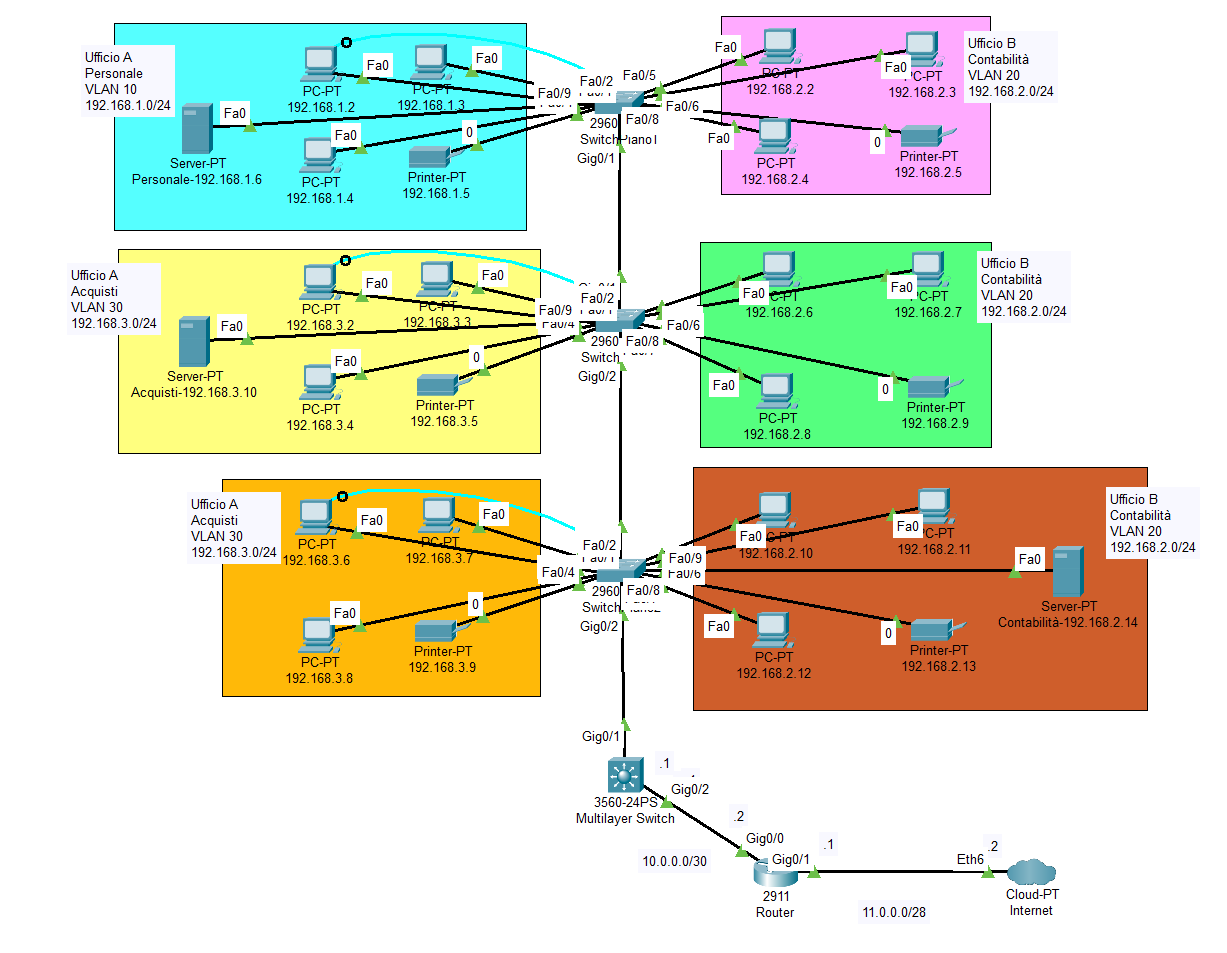
\includegraphics[width = 15cm]{Assets/MappaCompleta.png}
            \end{center}
        \end{figure}

    \subsection{Descrizione}
    \noindent Per la creazione della mappa, che vediamo in Figura \ref*{fig:mappa}, utilizziamo: 
        \begin{itemize}
            \item \textbf{3} \textit{Switch Layer 2}, modelli \textit{2960-24TT}, per i piani \textbf{T}, \textbf{1} e 
                \textbf{2};
            \item \textbf{1} \textit{Switch Layer 3}, modello \textit{3560-24PS}, per effettuare l'\textit{inter-vlan routing};
            \item \textbf{1} \textit{Router}, modello \textit{2911}, per effettuare l'accesso ad Internet.
        \end{itemize} 


    \newpage
    \section{Assegnamento e Indirizzamento}

    \subsection{Assegnamento delle VLAN}
    Le VLAN utilizzate sono:
        \begin{figure}[h!]
            \begin{center}
                \label{tab:TabellaVLAN}
                \caption{Tabella delle VLAN}
                ~ \\
                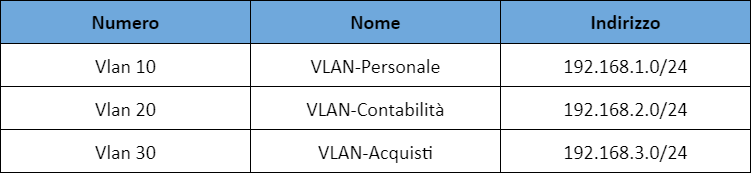
\includegraphics[width = 15cm]{Assets/TabellaDelleVlan.png}    
            \end{center}
        \end{figure}

    \subsection{Assegnamento Indirizzi}
    \noindent Dopo aver impostato le VLAN, come visto nella tabella \ref*{tab:TabellaVLAN}, impostiamo il piano di indirizzamento nella tabella \ref*{tab:indirizzamento}, 
        tramite il DHCP
        \begin{figure}[h!]
            \begin{center}
                \label{tab:indirizzamento}
                \caption{Piano di Indirizzamento}
                ~ \\ 
                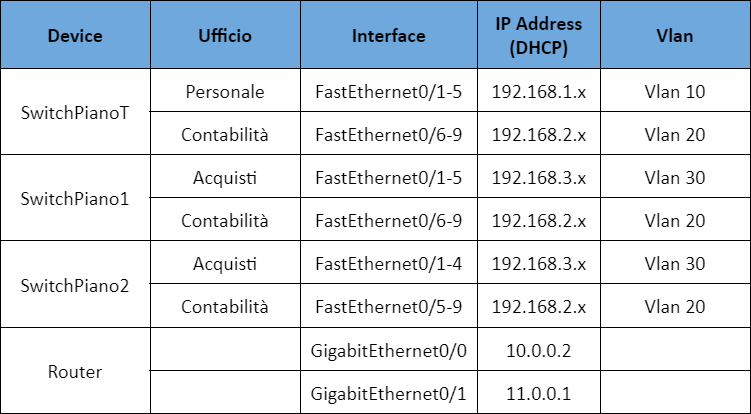
\includegraphics[width = 15cm]{Assets/TabellaDegliIndirizzi.png}
            \end{center}
        \end{figure}



    % II Page -- [Configurazione] %
    \newpage
    \fancyhead[L]{Configurazione}
   
    \section{Configurazione}
    Una volta assegnati gli indirizzi IP ai Device e ai PC/Stampanti/Sever, passiamo alla configurazione delle VLAN sugli Switch.
    
    \subsection{Configurazione - Switch Layer 2}
        \begin{center}
            Spegniamo le Interfacce non usate
            \begin{tcolorbox}[title=SwitchPianoT, colframe=gray!50!gray, colback=white!50!white]
                \begin{lstlisting}
#(config) interface range FastEthernet0/10-24
#(config-if-range) shutdown
                \end{lstlisting}
            \end{tcolorbox}
            Andiamo a definire le VLAN
            \begin{tcolorbox}[title=SwitchPianoT, colframe=gray!50!gray, colback=white!50!white]
                \begin{lstlisting}
#(config) VLAN 10
#(config-vlan) name VLAN-Personale
#(config-vlan) exit
#(config) VLAN 20
#(config-vlan) name VLAN-Contabilita
#(config-vlan) exit
#(config) VLAN 30
#(config-vlan) name VLAN-Acquisti
#(config-vlan) exit
                \end{lstlisting}
            \end{tcolorbox}
            Assegnamo le Interfacce alla VLAN. Quando una porta viene configurata come modalità access, significa che viene assegnata a una singola VLAN specifica e non trasmetterà il traffico di più VLAN come avviene sulle porte trunk.
            \begin{tcolorbox}[title=SwitchPianoT, colframe=gray!50!gray, colback=white!50!white]
                \begin{lstlisting}
#(config) interface range Fa0/1-5
#(config-if-range) switchport mode access
#(config-if-range) switchport access vlan 10

#(config) interface range Fa0/6-9
#(config-if-range) switchport mode access
#(config-if-range) switchport access vlan 20
                \end{lstlisting} 
            \end{tcolorbox}

            \newpage
            Infine impostiamo la porta trunk, la principale utilità di una porta trunk è quella di facilitare la comunicazione tra dispositivi appartenenti a diverse VLAN
            \begin{tcolorbox}[title=SwitchPianoT, colframe=gray!50!gray, colback=white!50!white]
                \begin{lstlisting}
#(config) interface GigabitEthernet0/1
#(config-if) switchport mode trunk
                \end{lstlisting} 
            \end{tcolorbox}
            Analogamente, ripetiamo le istruzioni appena descritte sugli altri 2 Switch L2 (Piano1 e Piano2). 
        \end{center}

    \subsection{Configurazione - Switch Layer 3}
        \begin{center}
            Prima di tutto abilitiamo il Routing sullo switch
            \begin{tcolorbox}[title=Multilayer Switch, colframe=gray!50!gray, colback=white!50!white]
                \begin{lstlisting}
#(config) ip routing
                \end{lstlisting}
            \end{tcolorbox}
            Andiamo a definire le VLAN che verranno instradate 
            \begin{tcolorbox}[title=Multilayer Switch, colframe=gray!50!gray, colback=white!50!white]
                \begin{lstlisting}
#(config) VLAN 10
#(config-vlan) name VLAN-Personale
#(config-vlan) exit
#(config) VLAN 20
#(config-vlan) name VLAN-Contabilita
#(config-vlan) exit
#(config) VLAN 30
#(config-vlan) name VLAN-Acquisti
#(config-vlan) exit
                \end{lstlisting}
            \end{tcolorbox}
            Creiamo le Interfacce virtuali
            \begin{tcolorbox}[title=Multilayer Switch, colframe=gray!50!gray, colback=white!50!white]
                \begin{lstlisting}
#(config) interface vlan 10
#(config-if) ip address 192.168.1.1 255.255.255.0

#(config) interface vlan 20
#(config-if) ip address 192.168.2.1 255.255.255.0

#(config) interface vlan 30
#(config-if) ip address 192.168.3.1 255.255.255.0
                \end{lstlisting} 
            \end{tcolorbox}

            \newpage
            Impostiamo la porta trunk abilitata per l'uso del protoccolo 802.1q. Quando si abilita una porta trunk per l'uso del protocollo 802.1Q, si sta configurando la porta per consentire il trasporto di dati appartenenti a più VLAN attraverso un singolo collegamento fisico. 
            \begin{tcolorbox}[title=Multilayer Switch, colframe=gray!50!gray, colback=white!50!white]
                \begin{lstlisting}
#(config) interface GigabitEthernet0/1
#(config-if) switchport mode trunk
#(config-if) switchport trunk encapsulation dot1q
                \end{lstlisting} 
            \end{tcolorbox}
            Per l'Interfaccia che "guarda" verso il Router per il collegamento ad Internet
            \begin{tcolorbox}[title=Multilayer Switch, colframe=gray!50!gray, colback=white!50!white]
                \begin{lstlisting}
#(config) interface GigabitEthernet0/2
#(config-if) no switchport
#(config-if) ip address 10.0.0.1 255.255.255.252
                \end{lstlisting} 
            \end{tcolorbox}
            Inseriamo la Rotta Statica di Default
            \begin{tcolorbox}[title=Multilayer Switch, colframe=gray!50!gray, colback=white!50!white]
                \begin{lstlisting}
#(config) ip route 0.0.0.0 0.0.0.0 10.0.0.2
                \end{lstlisting} 
            \end{tcolorbox}
            Inseriamo le Rotte Dinamiche 
            \begin{tcolorbox}[title=Multilayer Switch, colframe=gray!50!gray, colback=white!50!white]
                \begin{lstlisting}
#(config) Router Rip
#(config-router) network 10.0.0.0
#(config-router) network 192.168.1.0
#(config-router) network 192.168.2.0
#(config-router) network 192.168.3.0
                \end{lstlisting} 
            \end{tcolorbox}

            \newpage
            Definiamo i comandi per i pool DHCP, che è un protocollo di rete utilizzato per assegnare automaticamente indirizzi IP, 
                alle rispettive VLAN
            \begin{tcolorbox}[title=Multilayer Switch, colframe=gray!50!gray, colback=white!50!white]
                \begin{lstlisting}
#(config) ip dhcp pool poolVLANPersonale
#(dhcp-config) network 192.168.1.0 255.255.255.0
#(dhcp-config) default-router 192.168.1.1

#(config) ip dhcp pool poolVLANContabilita
#(dhcp-config) network 192.168.2.0 255.255.255.0
#(dhcp-config) default-router 192.168.2.1

#(config) ip dhcp pool poolVLANAcquisti
#(dhcp-config) network 192.168.3.0 255.255.255.0
#(dhcp-config) default-router 192.168.3.1
                \end{lstlisting} 
            \end{tcolorbox}
        \end{center}

    \newpage
    \subsection{Configurazione - Router}
    \begin{center}
        Configuriamo l'Interfaccia che "va" verso lo Switch L3
        \begin{tcolorbox}[title=Router, colframe=gray!50!gray, colback=white!50!white]
            \begin{lstlisting}
#(config) interface GigabitEthernet0/0
#(config-if) ip address 10.0.0.2 255.255.255.252
            \end{lstlisting}
        \end{tcolorbox} 
        Passiamo a quella che "va" verso Internet
        \begin{tcolorbox}[title=Router, colframe=gray!50!gray, colback=white!50!white]
            \begin{lstlisting}
#(config) interface GigabitEthernet0/1
#(config-if) ip address 11.0.0.1 255.255.255.240
\end{lstlisting}
        \end{tcolorbox}
        Inseriamo la Rotta Statica di Default
            \begin{tcolorbox}[title=Multilayer Switch, colframe=gray!50!gray, colback=white!50!white]
                \begin{lstlisting}
#(config) ip route 0.0.0.0 0.0.0.0 11.0.0.2
                \end{lstlisting} 
            \end{tcolorbox}
            Inseriamo le Rotte Dinamiche 
            \begin{tcolorbox}[title=Router, colframe=gray!50!gray, colback=white!50!white]
                \begin{lstlisting}
#(config) Router Rip
#(config-router) network 11.0.0.0
                \end{lstlisting}    
            \end{tcolorbox}
    \end{center}
\end{document}